\chapter{Background}
This chapter provides foundational background for numerical optimization, trajectory optimization, rigid-body dynamics with contact, predictive control, and implicit differentiation.

\section{Numerical Optimization}
Problems from every field of research can be formulated as numerical optimization problems. A myriad of algorithms have been designed to solve these problems ranging from grid search to derivative-free black-box methods to large-scale first-order gradient methods to efficient second-order approaches based on Newton's method. This thesis primarily focuses on constrained optimization with second-order methods for modeling dynamical systems, planning trajectories to generate useful behaviors, and control for robotic systems.

\paragraph{Problem.}
A canonical representation:
\begin{equation}
	\begin{array}{ll}
		\underset{x}{\mbox{minimize }}  & c(x) \\
		\mbox{subject to } & g(x) = 0, \\
		& h(x) \in \mathcal{K},
	\end{array} \label{intro_optimization_problem}
\end{equation}
has decision variables $x \in \mathbf{R}^n$, objective $c : \mathbf{R}^n \rightarrow \mathbf{R}$, equality constraints $g : \mathbf{R}^n \rightarrow \mathbf{R}^m$, and cone constraints $h : \mathbf{R}^n \rightarrow \mathbf{R}^p$ in the Cartesian product of cones $\mathcal{K}$. 

The designer formulates their problem \eqref{intro_optimization_problem} and a numerical optimizer searches for a solution $x^*$ that minimizes the objective while satisfying each of the constraints.

In the non-convex setting, there are limited guarantees that the optimizer will find the globally optimal solution, and for challenging problems, even converge to a locally optimal solution. For the robotics applications explored in this work, modeling non-smooth rigid-body dynamics with contact and fast optimization for control, these difficulties are of paramount importance.

\section{Trajectory Optimization}
Many optimization problems are of a temporal nature, for example, planning state and action sequences for robot motion planning. It is possible to exploit this structure with specialized numerical solvers and significantly reduce the computation complexity of optimizing such problems.

\paragraph{Problem.}
The trajectory optimization problem is formulated as:
\begin{equation}
	\begin{array}{ll}
		\underset{x_{1:T}, u_{1:T-1}}{\mbox{minimize }} & c_T(x_T) + \sum \limits_{t = 1}^{T-1} c_t(x_t, u_t)\\
		\mbox{subject to } & f_t(x_t, u_t) = x_{t+1},\phantom{\mathcal{K},} \, \quad t = 1,\dots,T-1,\\
		& g_t(x_t, u_t) = 0,\phantom{\,_{t+1}\mathcal{K}_t}\quad t = 1, \dots, T,\\
		& h_t(x_t, u_t) \in \mathcal{K}_t,\phantom{\,x_{t+1}}\quad t = 1, \dots, T, \label{intro_trajopt}\\
	\end{array}
\end{equation}
for a dynamical system with state $x_t \in \mathbf{R}^{n_t}$, control inputs $u_t \in \mathbf{R}^{m_t}$, time index $t$, discrete-time dynamics $f_t : \mathbf{R}^{n_t} \times \mathbf{R}^{m_t} \rightarrow \mathbf{R}^{n_{t+1}}$, and stage-wise objective $c_t: \mathbf{R}^{n_t} \times \mathbf{R}^{m_t} \rightarrow \mathbf{R}$,  equality constraints $g_t : \mathbf{R}^{n_t} \times \mathbf{R}^{m_t} \rightarrow \mathbf{R}^{p_t}$, and cone constraints $h_t : \mathbf{R}^{n_t} \times \mathbf{R}^{m_t} \rightarrow \mathbf{R}^{q_t}$, 
with the Cartesian product of convex cones $\mathcal{K}_t$, over a planning horizon $T$.

For robot dynamics and planning, problems with sizes on the order of hundreds to tens of thousands of decision variables can be efficiently optimized with second-order optimization algorithms, based on Newton's method. However, na\"{\i}ve algorithms will have cubic complexity in the planning horizon, state, action, and constraint dimensions.

Fortunately, certain problem formulations and specialized numerical solvers can greatly reduce this complexity, enabling online optimization in many cases.

\section{Finite-Horizon Linear Quadratic Regulator}
The canonical linear quadratic regulator (LQR) problem is a trajectory optimization problem \eqref{intro_trajopt} with affine dynamics and a quadratic objective. This convex quadratic program \cite{boyd2004convex} can be solved efficiently using an algorithm derived from dynamic programming \cite{bellman1966dynamic}.

\paragraph{Problem.}
The LQR problem:
\begin{align}
	\label{intro_lqr_problem}
	\underset{x_{1:T}, \phantom{\,} u_{1:T-1}}{\text{minimize }} & \quad  \frac{1}{2} x_T^T W_T x_T + w_T^T x_T + \sum \limits_{t = 1}^{T-1} \frac{1}{2} x_t^T W_t x_t + w_t^T x_t + \frac{1}{2} u_t^T R_t u_t + r_t^T u_t + x_t^T H_t u_t \\
	\text{subject to } & \quad x_{t+1} = A_t x_t + B_t u_t + C_t, \quad t = 1,\dots,T-1, \notag \\
	& \quad (x_1 \, \text{given}), \notag 
\end{align}
was originally formulated by Kalman \cite{kalman1964lqr} and has problem data: $W_t \in \mathbf{S}_{+}^{n_t}, w_t \in \mathbf{R}^{n_t}, R_t \in \mathbf{S}_{++}^{m_t}, r_t \in \mathbf{R}^{m_t}, H_t \in \mathbf{R}^{n_t \times m_t}, A_t \in \mathbf{R}^{n_{t+1} \times n_t}, B_t \in \mathbf{R}^{n_{t+1} \times m_t}, C_t \in \mathbf{R}^{n_{t+1}}$, and $x_1 \in \mathbf{R}^{n_1}$ that are provided by the designer.

The globally optimal solution is represented as the following feedback policy: 
\begin{equation}
	u = \pi_t(x) = K_t x + k_t, \label{intro_lqr_policy}
\end{equation}
where:
\begin{align}
	K_t &= -(R_t + B_t^T P_{t+1} B_t)^{-1} (H_t^T + B_t^T P_{t+1} A_t), \label{intro_lqr_feedback} \\
	k_t &= -(R_t + B_t^T P_{t+1} B_t)^{-1} (r_t + B_t^T P_{t+1} C_t + B_t^T p_{t+1}). \label{intro_lqr_affine}
\end{align}
These terms (\ref{intro_lqr_feedback}, \ref{intro_lqr_affine}) are computed recursively using dynamic programming.

\paragraph{Dynamic programming solution.}
First, we assume that the value function has a quadratic form:
\begin{equation}
	V_t(x) = \frac{1}{2} x^T P_t x + p_t^T x,
\end{equation}
with $P_t \in \mathbf{S}_{++}^{n_t}$ and $p_t \in \mathbf{R}^{n_t}$. At the final time step $T$ the value function is determined:
\begin{align}
	P_T &= W_T, \\
	p_t &= w_T.
\end{align}
Now, in a backward fashion, the value function is computed at preceding time steps: 
\begin{multline}
	P_t = W_t + A_t^T P_{t+1} A_t + K_t^T (R_t + B_t^T P_{t+1} B_t) K_t \\
	+ K_t^T (H_t^T + B_t^T P_{t+1} A_t) + (H_t + A_t^T P_{t+1} B_t) K_t, \label{intro_cost_to_go_matrix}
\end{multline}
\begin{multline}
	p_t = w_t + A_t^T P_{t+1} C_t + A_t^T p_{t+1} + K_t^T (R_t + B_t^T P_{t+1} B_t) k_t \\
	+ K_t^T (r_t + B_t^T P_{t+1} C_t + B_t^T p_{t+1}) + (H_t + A_t^T P_{t+1} B_t) k_t. \label{intro_cost_to_go_vector}
\end{multline}
The feedback policy is then computed using the optimal value function.

\paragraph{Optimal trajectories.}
The optimal trajectory, $\tau = (x_1, u_1, \dots, x_T)$, and associated duals, $\Lambda = (\lambda_1, \dots, \lambda_{T-1})$, are computed via a closed-loop forward rollout of the dynamics using the optimal policy from the initial state $x_1$:
\begin{align}
	u_t &= K_t x_t + k_t, \\
	x_{t+1} &= A_t x_t + B_t u_t + C_t, \\
	\lambda_t &= P_t x_t + p_t.
\end{align}

\section{Iterative Linear Quadratic Regulator}
For non-convex trajectory optimization problems, Iterative LQR (iLQR) is an efficient algorithm that leverages solutions to LQR problems \eqref{intro_lqr_problem}.

\paragraph{Problem.}
The following instance:
\begin{equation}
	\begin{array}{ll}
		\underset{u_{1:T-1}}{\mbox{minimize}} & c_T(x_T) + \sum \limits_{t = 1}^{T-1} c_t(x_t, u_t) \label{intro_ddp}\\
		\mbox{subject to} & x_{t+1} = f_t(x_t,u_t), \quad t = 1,\dots,T-1,\\
		& (x_1~\mbox{given}),
	\end{array}
\end{equation}
has (potentially) non-convex discrete-time dynamics and costs. The algorithm requires twice differentiable objective and dynamics, and utilizes derivatives of these functions. Additionally, only the controls are optimized and the state trajectory is recovered via forward rollouts.

\paragraph{Backward pass.}
A Taylor series approximates the objective to second order and the dynamics to first order about a nominal trajectory, $\bar{\tau} = (\bar{x}_1, \bar{u}_1, \dots, \bar{x}_T)$, denoted with an overbar ($\bar{\phantom{x}}$). This expansion is utilized as problem data: 
\begin{align}
	W_t &= [c_t]_{xx}(\bar{x}_t, \bar{u}_t), \\
	R_t &= [c_t]_{uu}(\bar{x}_t, \bar{u}_t), \\
	H_t &= [c_t]_{xu}(\bar{x}_t, \bar{u}_t), \\
	w_t &= [c_t]_{x}(\bar{x}_t, \bar{u}_t), \\
	r_t &= [c_t]_{u}(\bar{x}_t, \bar{u}_t), \\
	A_t &= [f_t]_{x}(\bar{x}_t, \bar{u}_t), \\
	B_t &= [f_t]_{u}(\bar{x}_t, \bar{u}_t), \\
	C_t &= 0,
\end{align}
to solve an LQR problem \eqref{intro_lqr_problem}.  

\paragraph{Forward pass.}
The resulting LQR feedback policy \eqref{intro_lqr_policy} is then utilized to rollout the dynamics from an initial state $x_1$: 
\begin{align}
	u_t &= \bar{u}_t + K_t (x_t - \bar{x}_t) + \alpha k_t, \\
	x_{t+1} &= f_t(x_t, u_t).
\end{align}
Importantly, because the expansion used to solve the LQR problem is only valid in a (potentially small) region around the nominal trajectory, which is not known \textit{a priori}, a line search over the parameter $\alpha \in [0, 1]$ is performed.

The trajectory with the lowest cost defined by the objective is selected as the new nominal trajectory, i.e., $\bar{\tau} \leftarrow \tau$. The procedure of alternating backward and forward passes is typically performed repeatedly until the change in objective value between iterations becomes small or a desired objective value is achieved.

\section{Rigid-Body Dynamics with Contact}
Non-smooth rigid-body dynamics with contact can be posed as a complementarity problem \cite{stewart1996implicit}. In this formulation, both impacts and friction are modeled as constraints on the system's configuration and contact impulses.

\paragraph{Impact.} For a system with a single contact point, we define a configuration-dependent signed-distance function, $\phi : \mathbf{Q} \rightarrow \mathbf{R}$:
\begin{equation} 
	\phi(q) \geq 0. \label{intro_sdf}
\end{equation}
An impact impulse with magnitude $\gamma \in \mathbf{R}$ is applied at the contact points in the direction of the surface normal in order to enforce \eqref{intro_sdf} and prevent interpenetration. A non-negative constraint:
\begin{align}
	\gamma \geq 0, \label{intro_impact_inequality}
\end{align}
enforces physical behavior that an impulse is repulsive (e.g., the floor does not attract bodies), and the complementarity condition:
\begin{align}
	\gamma \cdot \phi(q) = 0, \label{intro_impact_complementarity}
\end{align}
encodes switching behavior, e.g., enforcing zero force if the body is not in contact and allows non-zero force during contact.

\paragraph{Friction.} 
\begin{figure}[t]
	\centering
	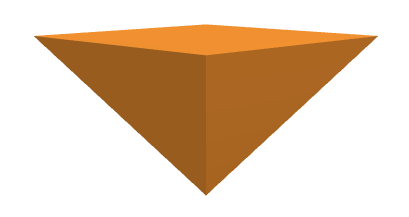
\includegraphics[width=0.25\columnwidth]{dojo/linearized_cone.png}
	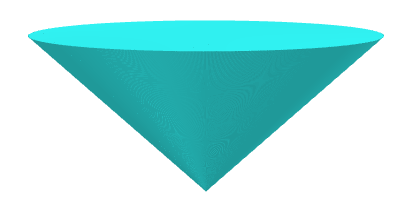
\includegraphics[width=0.25\columnwidth]{dojo/nonlinear_cone.png}
	\hfill
	\caption[Linearized and second-order friction-cone comparison]{Friction-cone comparison. Linearized double-parameterized (left) and nonlinear second-order (right) cones.}
	\label{intro_friction_cone_comparison}
\end{figure}
Coulomb friction \cite{moreau2011unilateral} models stick-slip behavior with friction that instantaneously maximizes the dissipation of kinetic energy between two objects in contact while remaining within a friction-cone. For a single contact point, this physical phenomenon can be modeled by the following optimization problem:
\begin{equation}
	\begin{array}{ll}
		\underset{b}{\mbox{minimize}} & \nu^T b\\
		\mbox{subject to} &\|b\|_2\leq \mu \gamma, \\
	\end{array} \label{intro_mdp}
\end{equation}
where $\nu \in \mathbf{R}^{2}$ is the tangential velocity at the contact point, $b \in \mathbf{R}^2$ is the friction force, and $\mu \in \mathbf{R}_{+}$ is the coefficient of friction between two objects \cite{moreau2011unilateral}. 

This problem is naturally a convex second-order cone program, and can be efficiently and reliably solved \cite{lobo1998applications}. However, classically, an approximate version of \eqref{intro_mdp}:
\begin{equation}
	\begin{array}{ll}
		\underset{\beta}{\mbox{minimize}} & \nu^T D^T \beta \\
		\mbox{subject to} & \beta^T \textbf{1} \leq \mu \gamma, \\
		& \beta \geq 0, \\
	\end{array} \label{intro_mdp_linear}
\end{equation}
formulated as a linear program, is instead solved. Here, the friction cone is linearized, (Fig. \ref{intro_friction_cone_comparison}) and the friction vector, $\beta \in \mathbf{R}^{2 d}$, is over parameterized and subject to additional non-negative constraints \cite{stewart1996implicit}, and $D \in \mathbf{R}^{2d \times 2}$ is the parameterization mapping. Finer discretization (i.e., larger $d$) of the friction cone can be utilized to better approximate the original problem, at the expense of a larger and computationally more expensive optimization problem.

The optimality conditions for \eqref{intro_mdp_linear} are:
\begin{align}
	\psi \cdot [\mu \gamma - \textbf{1}^T \beta] &= 0, \label{intro_friction_velocity_complementarity}\\
	\beta \circ [D \nu - \psi \textbf{1}] &= 0, \label{intro_friction_impulse_complementarity}\\
	\psi, \beta, [\mu \gamma - \textbf{1}^T \beta], [D \nu - \psi \textbf{1}] & \geq 0 \label{intro_friction_inequality}, 
\end{align}
where $\psi \in \mathbf{R}$ is a dual variable that can be interpreted as the magnitude of the contact-point tangential velocity, $\textbf{1}$ is a vector of ones, and $\circ$ is an element-wise product.

The primary drawback to this formulation is that the optimized friction force will naturally align with the vertices of the cone approximation, which may not align with the velocity vector of the contact point. This can lead to simulation artifacts such as creep. The reason this set of constraints is often preferred in practice is because they satisfy the requirements for a linear complementarity problem.

\paragraph{Linear complementarity problem.}
Contact dynamics are classically simulated with a velocity-based
time-stepping scheme formulated as a linear complementarity problem (LCP). This formulation combines the system's smooth dynamics with impact (\ref{intro_sdf}-\ref{intro_impact_complementarity}) and friction constraints (\ref{intro_friction_velocity_complementarity}-\ref{intro_friction_inequality}) in order to optimize the next velocity, $v \in \mathbf{R}^{n_v}$ of the system by finding the physically correct contact impulses, $\lambda = (\beta, \gamma)$. The next configuration $q \in \mathbf{R}^{n_q}$ is recovered from the solution: $q = q_{-} + h v$. Values at the previous time step are indicated with negative subscripts ($_{-}$). For a single contact point, dynamics are formulated as follows: 
\begin{align}
	\label{intro_feas_prob}
	{\mbox{find}} \quad & v, \lambda, \psi \\
	\mbox{subject to} \quad & M(q_{-}) (v - v_{-}) / h + C(q_{-}, v_{-}) = J(q_{-})^T \lambda, \notag \\
	& \gamma \circ [\phi(q_{-}) + \phi_q(q_{-}) \cdot h v] = 0, \notag\\
	& \psi \cdot \left[\mu \gamma - \textbf{1}^T \beta \right] = 0, \notag \\
	& \beta \circ [D J(q_{-}) v + \psi \textbf{1}] = 0, \notag\\
	& \phi, \gamma, [\mu \gamma - \textbf{1}^T \beta], [D J(q_{-}) v + \psi \textbf{1}], \beta, \psi \geq 0, \notag
\end{align}
where $M \in \mathbf{S}_{++}^{n_v}$ is the mass matrix, $C \in \mathbf{R}^{n_v}$ is the dynamics bias, $J \in \mathbf{R}^{(2d + 1) \times n_v}$ is the contact Jacobian that maps impulses at the contact point into the velocity space, and $h \in \mathbf{R}_{++}$ is the time step. The terms $M$, $C$, and $J$ are evaluated at the previous configuration, and a first-order approximation of the signed distance function at the previous configuration is utilized. This formulation generalizes to multiple contacts. 

Specialized solvers exist for LCPs. Typically, these optimizers rely on active-set methods that utilize pivoting algorithms to search the space of valid complementarity conditions \cite{dirkse1995path}.

\section{Contact-Implicit Trajectory Optimization}
Direct trajectory optimization can utilize the LCP contact dynamics formulation to plan trajectories for systems that make and break contact with their environment \cite{posa2014direct} without requiring hybrid dynamics \cite{westervelt2003hybrid} or explicitly enumerating all of the possible sequences of contact configurations. This enables the optimizer to potentially generate motion plans without pre-specified contact plans using task-level specifications via an objective.
 
\paragraph{Problem.} The contact-implicit trajectory optimization problem:
\begin{align}
	\underset{\substack{x_{1:T}, u_{1:T-1}, \\ \lambda_{1:T-1}, \psi_{1:T-1}}}{\mbox{minimize }} & c_T(x_T) + \sum \limits_{t = 1}^{T-1} c_t(x_t, u_t) \label{intro_ci_trajopt}\\
	\mbox{subject to} & \quad M(q_{t}) (v_{t+1} - v_{t}) / h + C(q_t, v_t) -B(q_{t}) u - J(q_{t})^T \lambda_t = 0, \quad t = 1,\dots,T-1, \notag \\
	& \quad q_t + h v_{t+1} - q_{t+1} = 0, \quad \quad \, \, \, \, \quad \quad \quad \quad \quad \quad \quad \quad \quad \quad \quad \quad \quad \, \, t = 1,\dots,T-1, \notag \\
	& \quad \gamma_t \circ \phi(q_{t+1}) = 0, \notag \quad \quad \quad \quad \, \, \, \, \, \, \, \quad \quad \quad \quad \quad \quad \quad \quad \quad \quad \quad \quad \quad \, \, t = 1,\dots,T-1, \notag\\
	& \quad \psi_t \cdot \left[\mu \gamma_t - \textbf{1}^T \beta_t \right] = 0, \, \, \,  \, \, \quad \quad \quad \quad \quad \quad \quad \quad \quad \quad \quad \quad \quad \quad \quad \, \, t = 1,\dots,T-1, \notag \\
	& \quad \beta_t \circ [D J(q_{t}) v_{t+1} + \psi_t \textbf{1}] = 0, \, \quad \quad \quad \quad \quad \quad \quad \quad \quad \quad \quad \quad \quad \, t = 1,\dots,T-1, \notag\\
	& \quad \phi(q_{t+1}), \gamma_t, [\mu \gamma_t - \textbf{1}^T \beta], [D J(q_{t}) v_{t+1} + \psi_t \textbf{1}], \beta_t, \psi_t \geq 0, \quad \quad t = 1,\dots,T-1, \notag \\
	& \quad (x_1 \, \mbox{given}) \notag,
\end{align}
with states, $x = (q, v)$, directly encodes the LCP constraints and aims to minimize an objective. This formulation generalizes to multiple contacts. 

\paragraph{Complementarity reformulation.} To work well in practice with general-purpose off-the-shelf solvers for non-convex problems, the complementarity constraints are reformulated using an exact $\ell_1\mbox{-norm}$ penalty \cite{manchester2020variational}:
\begin{equation}
	\begin{array}{ll}
		\underset{}{\mbox{find }}  & a, b\\
		\mbox{subject to } & a \circ b = 0, \\ 
		& a, b \geq 0
	\end{array}
	\quad
	\rightarrow 
	\quad
	\begin{array}{ll}
		\underset{a, b, s}{\mbox{minimize }}  & \rho s\\
		\mbox{subject to } & s \mathbf{1} - a \circ b \geq 0, \\
		& a, b, s \geq 0
	\end{array} \label{intro_complementarity_reformulation}
\end{equation}
This formulation relaxes the complementarity constraints and empirically results in superior convergence properties. As $\rho \rightarrow \infty$, we have $s \rightarrow 0$, and the original formulation is recovered. Despite the reformulation's practical performance, it requires additional decision variables and careful selection of the initial penalty parameter, $\rho \in \mathbf{R}_+$.

\section{Predictive Control}
A powerful tool for controlling complex systems is predictive control (PC) \cite{richalet1978model}. These algorithms leverage fast dynamics and planning algorithms to perform online optimization. This framework has been successfully deployed in numerous real-world settings including: control for chemical and nuclear processes \cite{na2003model, lopez2013fast}, navigation for autonomous vehicles \cite{falcone2007predictive}, and whole-body control of humanoid robots \cite{atlas2019parkour}.

In this framework, a model and the current state are utilized to predict the future evolution of the system under candidate action sequences. Numerical optimization is performed online to search for improved sequences. The best plan is utilized to control the system until a new (hopefully) improved plan has been computed.

\paragraph{Problem.}
The predictive control policy:
\begin{align}
	u \leftarrow \pi(x)
	\begin{cases}
		\begin{array}{ll}
			\underset{x_{1:T}, u_{1:T}}{\mbox{minimize }}  & \sum \limits_{t = 1}^{T} c_t(x_t, u_t) \\
			\mbox{subject to } & x_{t+1} = f_t(x_t, u_t),  \quad t = 1, \dots, T,\\
			& x_1 = x
		\end{array}
	\end{cases}
	\label{intro_mpc_policy}
\end{align}
is formulated as an optimization problem where $T$ is the planning horizon, typically much shorter than the horizon we care to control the system. The optimized action sequence is utilized to return an action from the policy. If replanning is performed at a high rate, the resulting sequence of open-loop plans will effectively perform feedback.

\paragraph{Practical enhancements.} There are three key enhancements for PC algorithms that lead to its practical performance. First, actions returned by the policy from approximate solutions to the internal optimization problem are often highly effective. As a result, since it is not necessary to solve the problem to convergence the computational burden is substantially reduced, enabling faster replanning, which typically leads to superior feedback. 

Second, myopic planning horizons are typically sufficient to achieve desired long-term behavior (i.e., minimizing total returns over the full planning horizon). This enables simpler models that may be easier to construct and less expensive to evaluate to be used during forward prediction since simulating accurate long-term behavior is not necessary. 

Third, the temporal nature of the control problem results in sequential policy evaluations that will solve similar optimization problems. As a result, warm starting, where the solution to a previous problem is used as a starting point for the current problem, can be effectively utilized. Employing this technique can greatly reduce the computational cost of policy evaluations.

\section{Augmented Lagrangian Method}
For equality-constrained problems, the augmented Lagrangian method \cite{bertsekas2014constrained} is a simple and effective algorithm, particularly when the problem is non-convex. This method transforms the constrained problem into an unconstrained form, then alternates between minimizing an augmented objective and performing updates to the dual variables and a penalty parameter.

\paragraph{Problem.}
An equality-constrained problem:
\begin{equation}
	\begin{array}{ll}
		\underset{x}{\mbox{minimize }}  & c(x) \\
		\mbox{subject to } & g(x) = 0, \\
	\end{array}
	\label{intro_equality_constrained}
\end{equation}
is transformed into an unconstrained problem by introducing dual variables, $\lambda \in \mathbf{R}^m$, and a quadratic penalty parameterized by $\rho \in \mathbf{R}_+$:
\begin{equation}
	L_{\mathcal{A}}(x; \lambda, \rho) = c(x) + \lambda^T g(x) + \frac{\rho}{2} g(x)^T g(x), 
	\label{intro_augmented_lagrangian}
\end{equation}
where we refer to $L_{\mathcal{A}}$ as the \emph{augmented Lagrangian} for the problem \eqref{intro_equality_constrained}.

\paragraph{Primal method.}
The classic method alternates between minimizing the augmented Lagrangian  \eqref{intro_augmented_lagrangian} and performing outer updates on the dual variables and penalty:
\begin{equation} 
	\lambda \leftarrow \lambda + \rho g(x), \quad \rho \leftarrow \phi (\rho), \label{intro_augmented_lagrangian_update}
\end{equation}
until a solution to the original problem \eqref{intro_equality_constrained} is found \cite{bertsekas2014constrained}. This typically requires ten or fewer outer updates and a simple update, $\phi : \mathbf{R}_+ \rightarrow \mathbf{R}_+$, that scales the penalty by a constant value, works well in practice.
Throughout, subscripts are used to denote derivatives and we drop the variable dependence of the functions for clarity. The KKT system for this method is:
\begin{equation} 
	\Big[c_{xx} + \rho g_x^T g_x + \sum \limits_{i = 1}^m (\lambda^{(i)} + \rho g^{(i)}) g_{xx}^{(i)} \Big] \Delta x = -\Big[c_x + g_x^T (\lambda + \rho g)\Big]. \label{intro_augmented_lagrangian_update} 
\end{equation}

Search directions $\Delta x \in \mathbf{R}^n$ are computed by solving the linear system \eqref{intro_augmented_lagrangian_update} for fixed values of the dual variables and penalty. Newton's method with a line search is utilized to compute iterates that satisfy the KKT conditions, or residual, to a desired tolerance.

While this simple algorithm is effective at finding low to medium quality solutions, the KKT matrix becomes increasingly ill-conditioned as the penalty is increased in order to achieve better satisfaction of the equality constraints, degrading the quality of the Newton step. As a result, this method is best suited for applications where finding approximate solutions quickly is desirable, but highly accurate solutions are unnecessary.

\paragraph{Primal-dual method.}
To address the deficiencies of the primal method, a primal-dual method introduces additional dual variables, $y \in \mathbf{R}^m$, and constraints:
\begin{equation}
	y = \lambda + \rho g(x), \label{intro_dual_constraint}
\end{equation}
in order to utilize an alternative KKT system with better numerical properties.

Combining these constraints \eqref{intro_dual_constraint} with the primal KKT system \eqref{intro_augmented_lagrangian_update} and performing a simple manipulation of the new equations yields 
the \textit{primal-dual} augmented-Lagrangian KKT system:
\begin{align}
	\setstackgap{L}{1.1\baselineskip}
	% \fixTABwidth{T}
	\bracketMatrixstack{
		c_{xx} + \sum \limits_{i = 1}^m y^{(i)} g_{xx}^{(i)} & g_x^T \\ 
		g_x & -\frac{1}{\rho} I
	}
	\bracketVectorstack{ 
		\Delta x \\ 
		\Delta y
	}
	= 
	-\bracketMatrixstack{ 
		c_x + g_x^T y \\ 
		g + \frac{1}{\rho}(\lambda - y) 
	}. \label{intro_augmented_lagrangian_primal_dual}
\end{align}
In contrast to the primal system \eqref{intro_augmented_lagrangian_update}, this system \eqref{intro_augmented_lagrangian_primal_dual} does not become ill-conditioned as the penalty is increased because this term does not appear in the KKT matrix---only its inverse appears (i.e., $-\frac{1}{\rho} I$), which actually enhances the conditioning of the system by performing dual regularization  \cite{kuhlmann2018primal,gill2012primal,argaez2002global}. Further, this method implicitly satisfies the linear independence constraint qualification (LICQ) \cite{nocedal2006numerical}, necessary for most second-order methods for constrained optimization, because the KKT matrix remains full rank even in cases where $g_x$ is rank deficient as a result of the dual regularization \cite{izmailov2012global}.

Additionally, the KKT conditions now contain relaxed constraints (i.e., $g(x) + \frac{1}{\rho}(\lambda - y))$ that are particularly helpful for complementarity constraints since these elements of the residual are only satisfied in the limit as outer updates are performed.

Similar to the primal method, search directions ($\Delta x, \Delta y$) are computed by solving the linear system \eqref{intro_augmented_lagrangian_primal_dual} for fixed values of the dual variables estimates and penalty. Newton's method with a line search is utilized to compute iterates that satisfy the KKT conditions, or residual, to a desired tolerance. Outer updates to the dual estimates and penalty parameter are performed as before.

\section{Interior-Point Method}
For problems with hundreds to tens of thousands of decision variables and cone constraints, interior-point methods are efficient and return highly accurate solutions.
\paragraph{Problem.}
A cone program:
\begin{equation}
	\begin{array}{ll}
		\underset{x}{\mbox{minimize }}  & c(x) \\
		\mbox{subject to } & x \in \mathcal{K}, \\
	\end{array}
	\label{intro_cone_program}
\end{equation}
minimizes an objective while satisfying a cone constraint. For robotics applications, common cones include the positive orthant (i.e., inequality constraints):
\begin{equation} 
	x^{(i)} \ge 0, \quad i = 1, \dots, n \quad \rightarrow \quad x \in \mathbf{R}^n_{+},
\end{equation}
and second-order cones:
\begin{equation}
	\|x^{(2:n)}\|_2 \leq x^{(1)} \quad \rightarrow \quad x \in \mathcal{Q}^n.
\end{equation}

\paragraph{Primal method.}
An interior-point method transforms the original constrained problem  \eqref{intro_cone_program} into an unconstrained form using a logarithmic barrier:
\begin{equation}
	L_{\mathcal{B}}(x; \kappa) = c(x) - \kappa \phi(x),
	\label{intro_barrier_function}
\end{equation}
where we refer to $L_{\mathcal{B}}$ as the \textit{barrier Lagrangian}. The barrier functions are:
\begin{equation}
	\phi(x) = \sum \limits_{i = 1}^n \mbox{log}(x^{(i)}),
\end{equation}
and 
\begin{equation}
	\phi(x) = \frac{1}{2} \mbox{log}\Big((x^{(1)})^2 - (x^{(2:n)})^T x^{(2:n)} \Big),
\end{equation}
for the positive orthant and second-order cone, respectively.

The classic method alternates between minimizing the barrier Lagrangian \eqref{intro_barrier_function} while taking steps that ensure the cone constraint remains satisfied, and outer updates to the central-path parameter, $\kappa \in \mathbf{R}_{+}$, until a solution to the original problem \eqref{intro_cone_program} is found \cite{boyd2004convex}. An effective strategy for the update is to decrease the parameter by a constant factor, $\kappa \rightarrow 0$. 

The KKT system for this method is:
\begin{equation}
	\Big[c_{xx} - \kappa \phi_{xx} \Big] \Delta x = -\Big[c_x - \kappa \phi_x \Big]. \label{intro_barrier_gradient}
\end{equation}
As the central-path parameter is decreased, the logarithmic barrier becomes a closer approximation to the indicator function, which has an infinite cost if a constraint is violated and is otherwise zero \cite{boyd2004convex}. While simple, this approach suffers from numerical ill-conditioning, similar to the primal augmented Lagrangian method, as the central-path parameter approaches zero, degrading a solver's ability to find accurate solutions to the original problem \eqref{intro_cone_program}.

\paragraph{Primal-dual method.} 
To address the conditioning issues of the primal method, additional dual variables, $z \in \mathbf{R}^n$, and complementarity constraints are introduced to form a new KKT system:
\begin{align} 
	\setstackgap{L}{1.25\baselineskip}
	\begin{bmatrix} 
		c_{xx} & -I \\ 
		\mbox{\textbf{diag}}(z)  & \mbox{\textbf{diag}}(x) 
	\end{bmatrix}
	\begin{bmatrix} 
		\Delta x \\ 
		\Delta z
	\end{bmatrix} &= 
	-
	\bracketMatrixstack{ 
		c_x - z \\
		x \circ z - \kappa \mathbf{e}
	}, \label{intro_interior_point_primal_dual}\\
	x \in \mathcal{K}, z &\in \mathcal{K}^* \label{intro_cone_primal_dual_cones}.
\end{align}
Similar to the primal-dual augmented Lagrangian method, this KKT matrix does not depend on the central-path parameter, resulting in significantly better numerical conditioning than primal methods. The complementarity constraints in the KKT conditions are relaxed (i.e., $x \circ z - \kappa \mathbf{e})$, only being satisfied in the limit as the central-path parameter is decreased to zero. For the positive orthant, the target $\mathbf{e} = \mathbf{1}$ and the cone product $\circ$ denotes an element-wise product. For the second-order cone, the target is: $\mathbf{e} = (1, 0^{(n-1)})$, with cone product: $a \circ b = (a^T b, \, a^{(1)} b^{(2:n)} + b^{(1)} a^{(2:n)})$ \cite{domahidi2013ecos, vandenberghe2010cvxopt}. Both cones are self dual \cite{boyd2004convex}, and $\mathcal{K} = \mathcal{K}^*$.

With the new system, search directions ($\Delta x, \Delta z$) are computed by solving the linear system \eqref{intro_interior_point_primal_dual} for fixed values of the central path parameter. Newton's method with a line search is utilized to compute iterates that satisfy the KKT conditions, or residual, to a desired tolerance, while respecting the cone constraints on the primal and dual variables. Updates to the central-path parameter are performed as before.

\section{Implicit Differentiation}
Many optimization problems can be formulated as finding a fixed point to an implicit function. An implicit function, $r : \mathbf{R}^a \times \mathbf{R}^b \rightarrow \mathbf{R}^a$, is defined as:
\begin{equation}
	r(w^*; \theta) = 0, \label{intro_implicit_function}
\end{equation}
for a fixed-point $w^* \in \mathbf{R}^a$ and problem data $\theta \in \mathbf{R}^b$. Further, it is often useful to compute the sensitivity of this solution with respect to the problem data, i.e., differentiate through the implicit function.

Computing this sensitivity is possible by applying the implicit-function theorem \cite{dini1907lezioni}. First, the function is approximated to first order at the solution:
\begin{equation}
	\cancelto{0}{r} + \frac{\partial r}{\partial w} \delta w + \frac{\partial r}{\partial \theta} \delta \theta = 0.
\end{equation}
Then, it is possible to solve for the relationship: 
\begin{equation}
	\frac{\partial w^*}{\partial \theta} = -\Big(\frac{\partial r}{\partial w}\Big)^{-1} \frac{\partial r}{\partial \theta}, \label{intro_solution_sensitivity}
\end{equation}
and recover the sensitivity.

Newton's method is typically employed to find solutions. When the method succeeds, the sensitivity \eqref{intro_solution_sensitivity} can be computed and the factorization of $\partial r / \partial w$ used to find the solution is reused to efficiently compute sensitivities at very low computational cost, using only back-substitution. In the case that $\partial r / \partial w$ is not full rank, an approximate solution, e.g., least-squares \cite{boyd2004convex}, can be computed, or regularization can be employed. Additionally, each element of the sensitivity can be computed in parallel.

\paragraph{Differentiating through an optimization problem.}
Implicit differentiation can also be used to compute the sensitivity of solutions, found by numerical optimizers, with respect to the optimization problem data. Numerical solvers find fixed points, comprising primal and dual variables, to the gradient of the problem's Lagrangian. This approach has been successfully applied to quadratic programs \cite{amos2017optnet}, and more generally, convex cone programs \cite{agrawal2019differentiating}.

While it is possible to compute derivatives via finite-difference schemes, this approach requires at least as many calls to the solver as there are problem data elements. An alternative approach to computing gradients through a solver is to unroll the algorithm and utilizing the chain rule to differentiate sequentially through each iteration \cite{domke2012generic}. However, in practice, this approach requires truncating the number of iterates, which can lead to low-accuracy solutions, and this approach can be plagued by numerical issues that lead to exploding or vanishing gradients. Implicit differentiation is generally more efficient and able to return highly accurate sensitivities. 




